\documentclass{beamer}
\usepackage{presentation}

\begin{document}

\frame{\titlepage}

\begin{frame}
  \frametitle{Need and goal statement}
  \textbf{Need Statement}:
  \input{build/need_statement_md}
  \newline
  \newline
  \textbf{Goal Statement}:
  \input{build/goal_statement_md} \\
\end{frame}

\begin{frame}
  \frametitle{Design Objectives}
  Four key objectives:
  \begin{itemize}
    \item Presence
    \item Portability / ease of set-up
    \item Configurable
    \item Accessible
  \end{itemize}

  \note{This is a note}
\end{frame}

\begin{frame}
  \frametitle{What our project could have been...}
  % TODO
  We considered several ideas to address our goal statement after analyzing existing methods:
  \\~\\
  \begin{columns}
    \column{0.5\textwidth}
    Method
    \begin{itemize}
      \item Personal assistant
      \item Accountability
      \item Notification
      \item Planner
    \end{itemize}

    \column{0.5\textwidth}
    Device
    \begin{itemize}
      \item Game device
      \item Face tracking water sprayer
      \item Home assistant
      \item PDA Device
    \end{itemize}

  \end{columns}

  \note{This is a note}
\end{frame}

\begin{frame}
  \frametitle{Choosing the best design}
  % TODO
  We derived weights from
  \begin{longtable}[]{@{}ll@{}}
  \toprule
  Criteria & Weight \\
  \midrule
  \endhead
  Budget & 20 \\
  Presence & 20 \\
  Ease of Use & 20 \\
  Barrier of Entry & 20 \\
  Sustainability & 10 \\
  Privacy & 10 \\
  \bottomrule
  \end{longtable}

  Top designs: game device, tablet-sized planner, PDA device

  \note{This is a note}
\end{frame}

\begin{frame}
  \frametitle{Planning: CPM \& Gantt chart}
  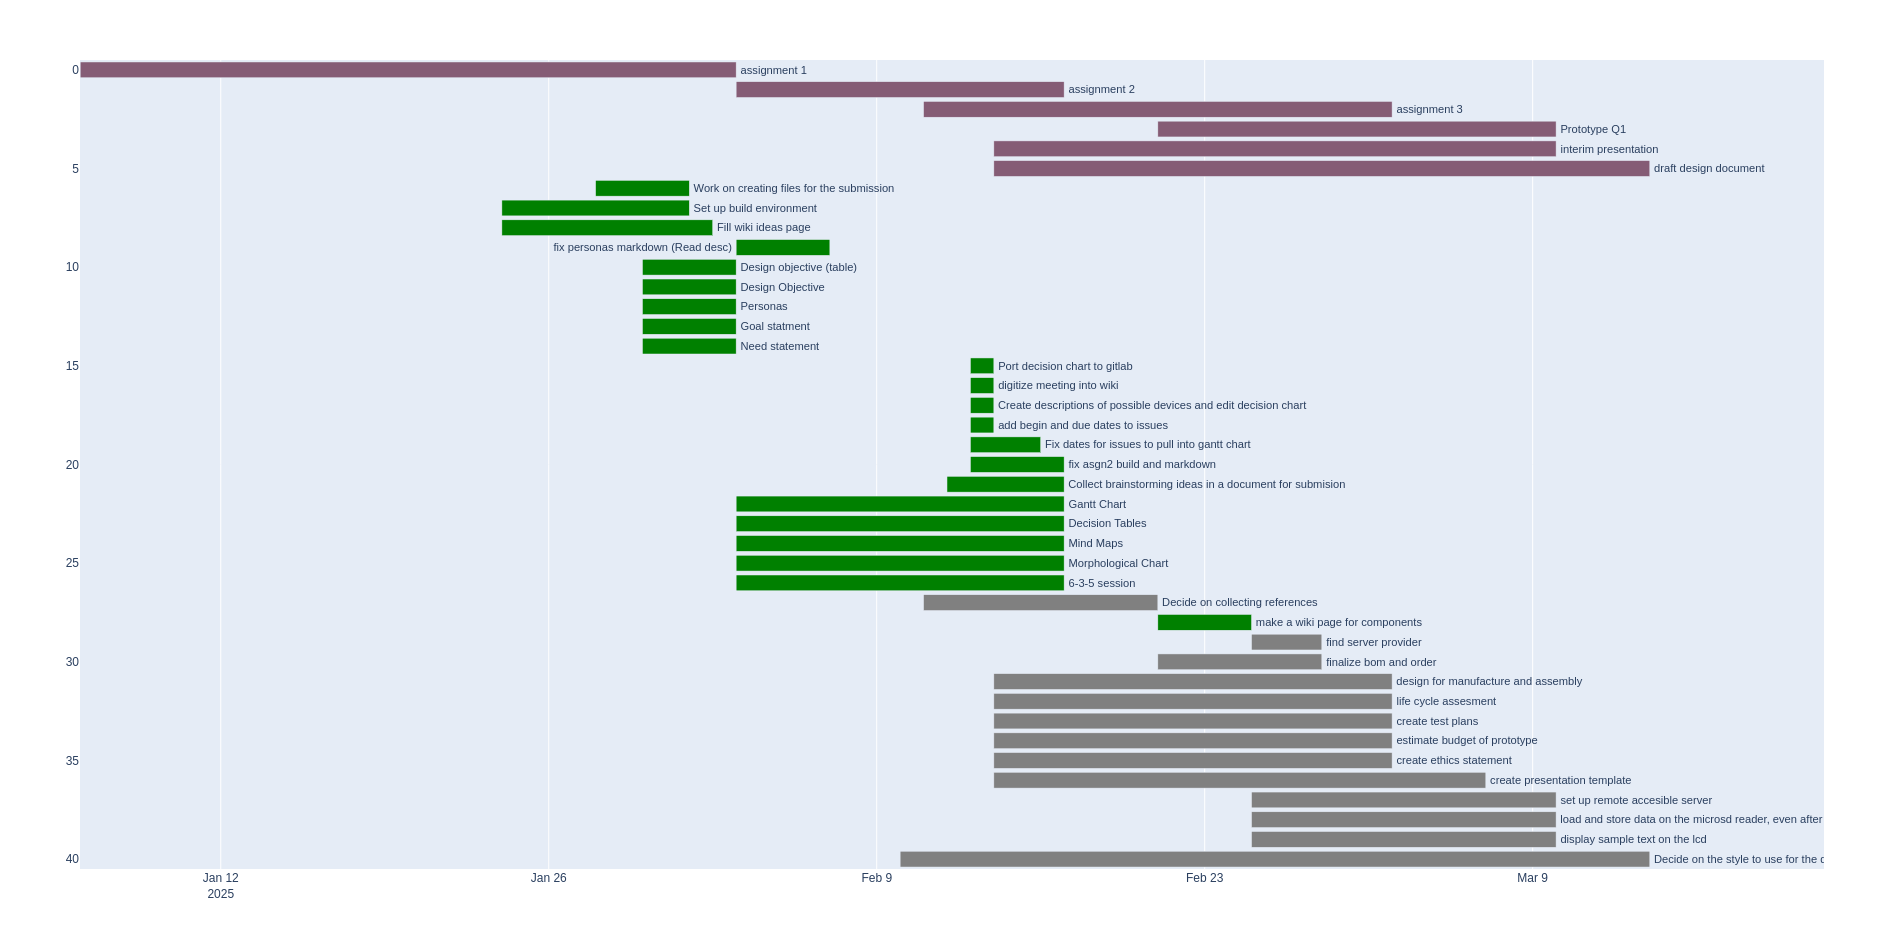
\includegraphics[width=\textwidth]{gantt.png}
  The gantt chart was generated from gitlab issues.

  \note{This is a note}
\end{frame}

\begin{frame}
  \frametitle{Testing}

  \begin{columns}
    \column{0.7\textwidth}
    Testing on the microcontroller can be automated with Unity and pytest.
    \\~\\
    For physical and software tests, we will define the following:
    \begin{itemize}
      \item Stimulus
      \item Control variables
      \item Expected Results
      \item Walkthrough of the procedure
    \end{itemize}

    \column{0.3\textwidth}
    
\includegraphics[width=0.5\textwidth]{pytest_logo.png} \\
    
\includegraphics[width=0.5\textwidth]{unity_logo.png}

  \end{columns}
  \hfill {\tiny Source: pytest docs, Unity homepage}
  \note{This is a note}
\end{frame}

% --- Prototyping ---
\begin{frame}
  \frametitle{Prototype}
  \begin{columns}
    \column{0.5\textwidth}
    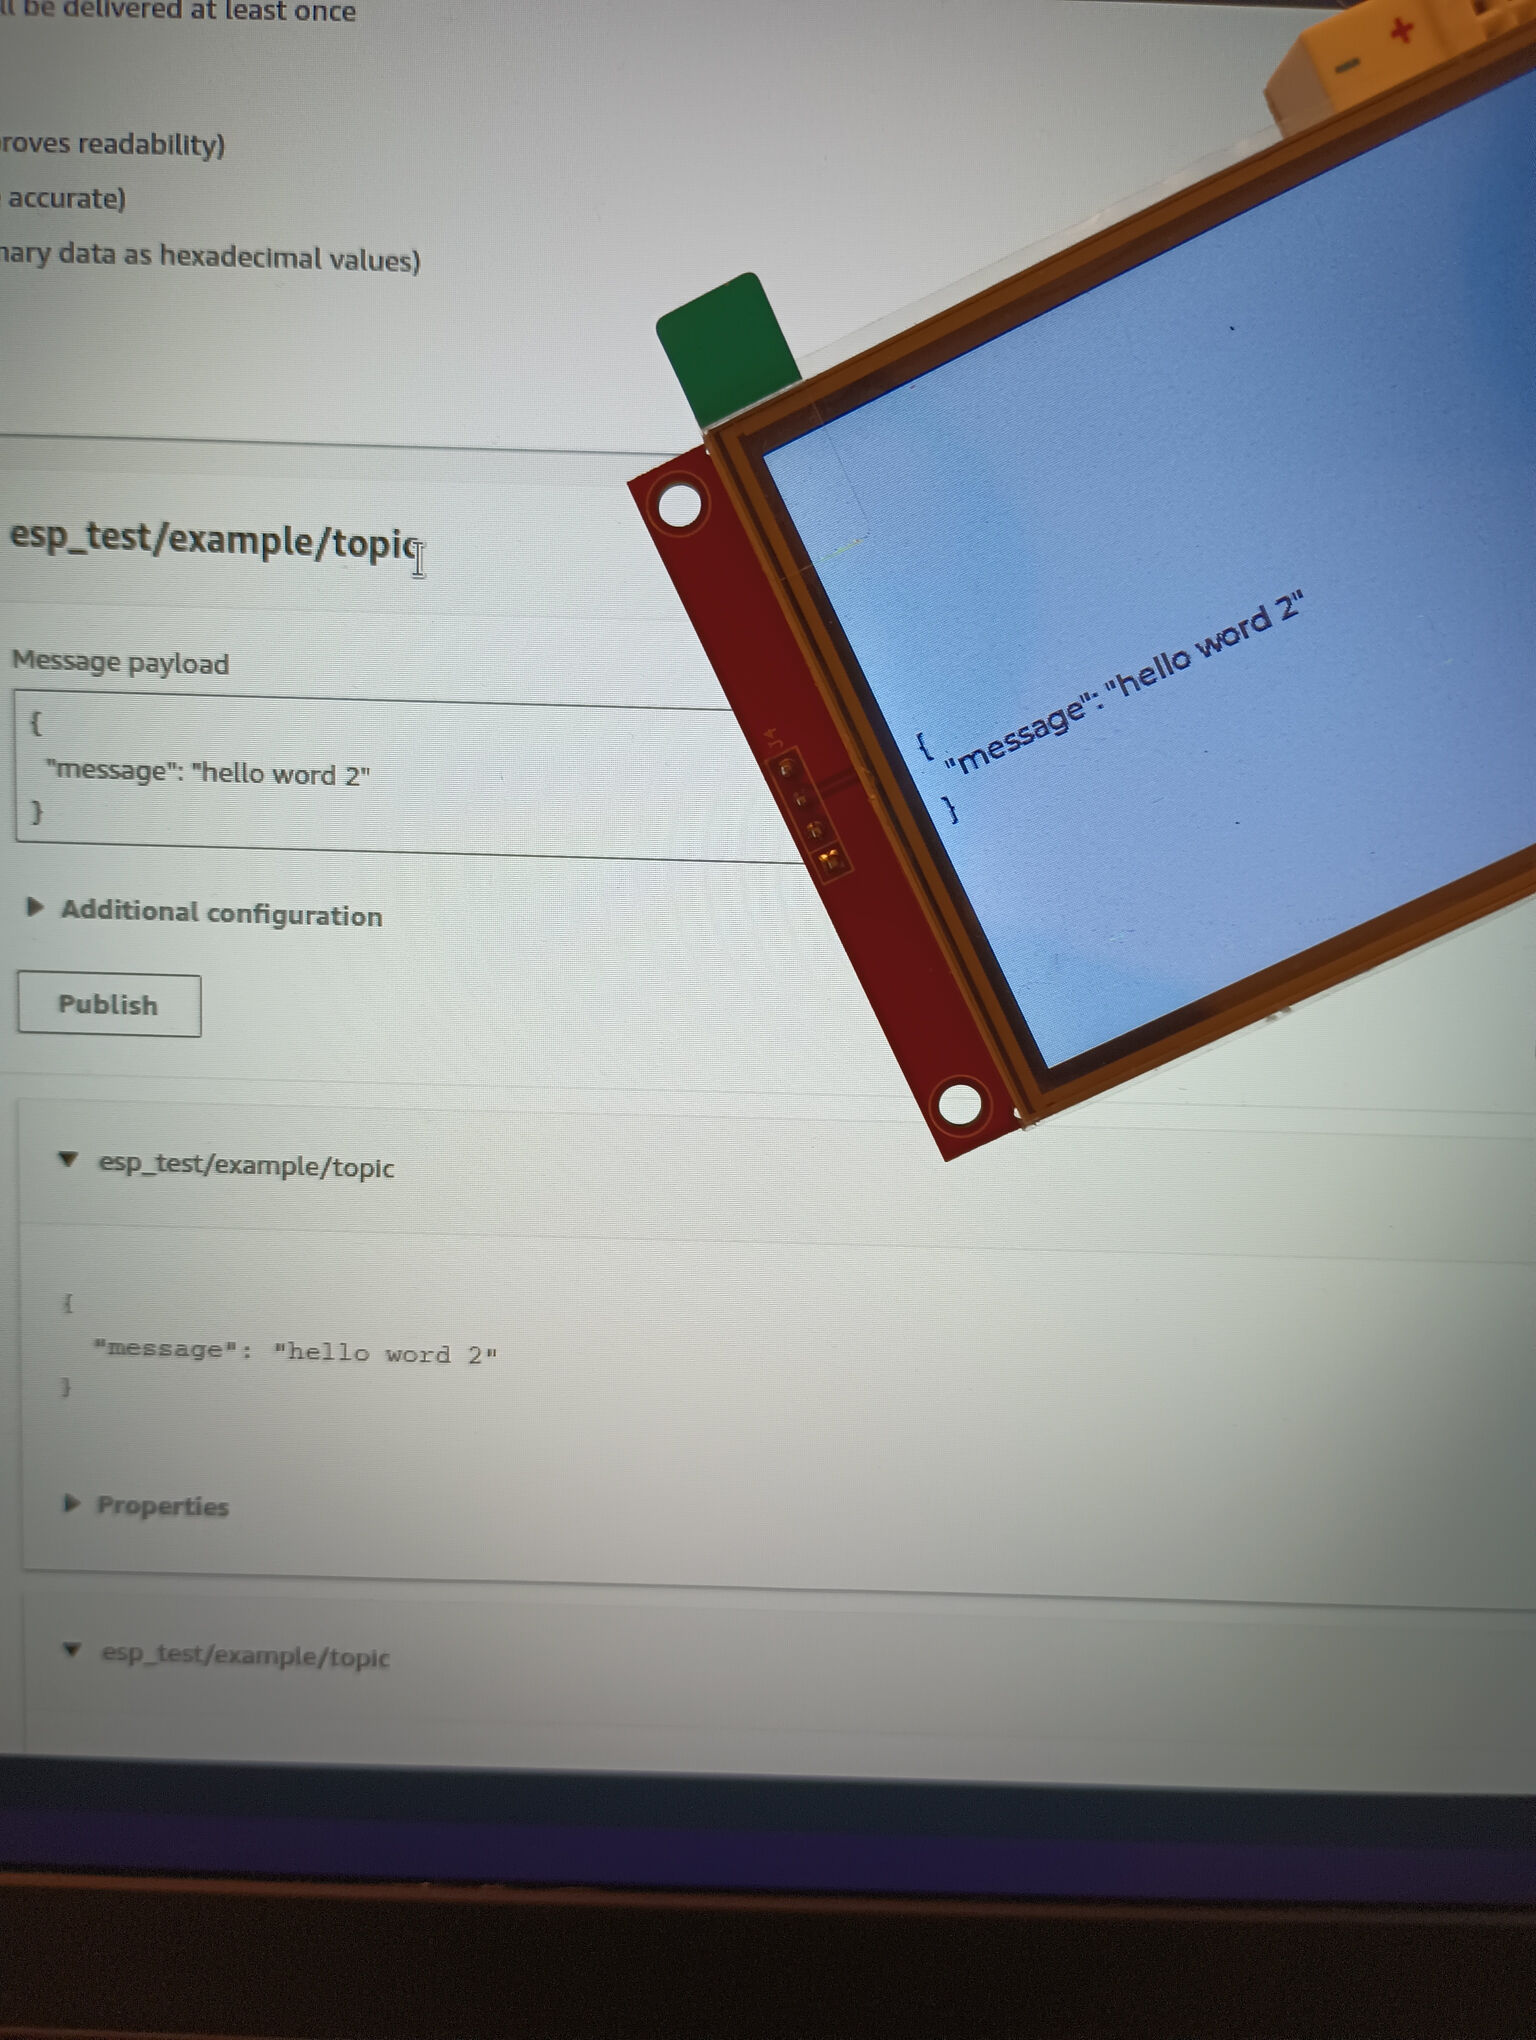
\includegraphics[height=0.7\textheight]{aws_demo.jpg}
    \column{0.5\textwidth}
    Functionality is spread across three tasks, the latter two running concurrently
    \begin{enumerate}
      \item app\_main
      \item AWS IoT connection
      \item LCD screen updates
    \end{enumerate}
  \end{columns}
  \hfill {\tiny Source: pytest Apple Playground}

  \note{This is a note}
\end{frame}

\begin{frame}
  \frametitle{Embedded System Flow}
  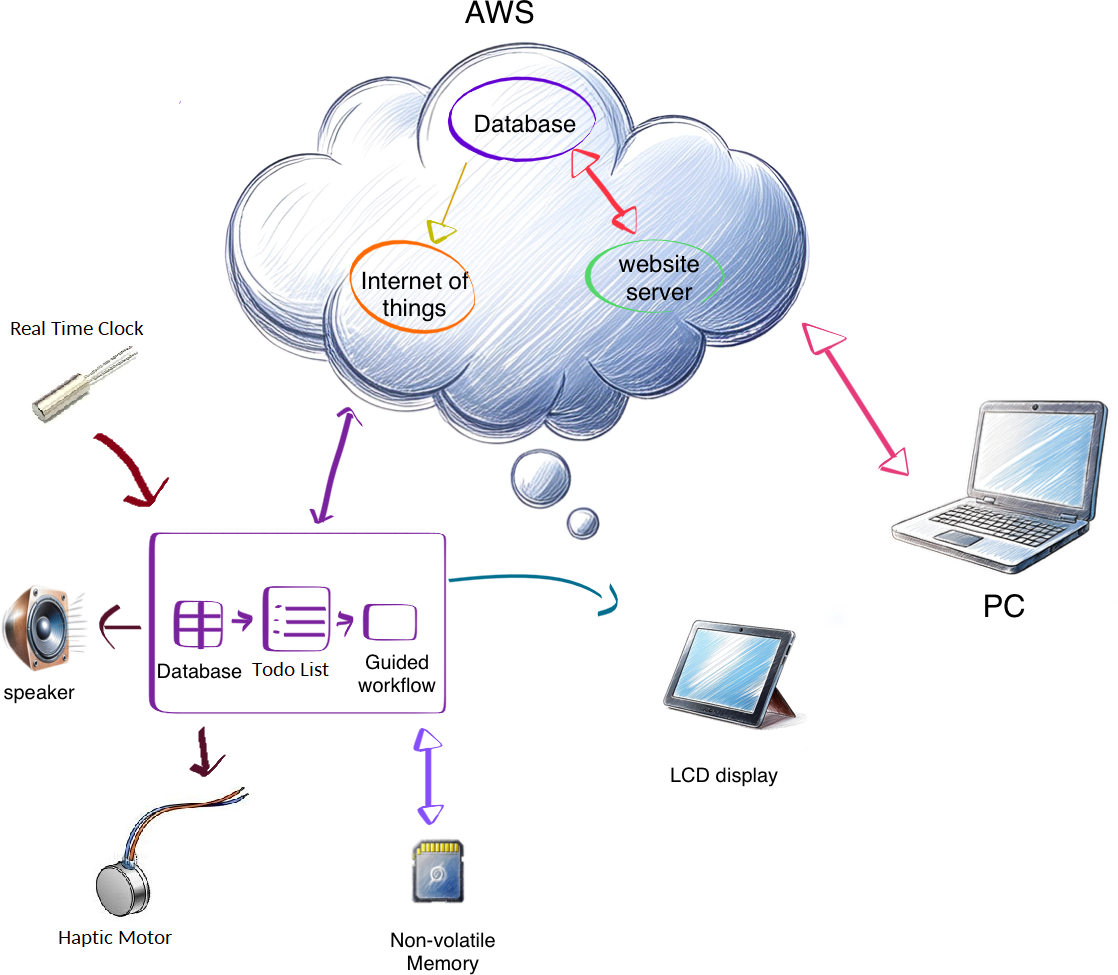
\includegraphics[width=\textwidth]{embedded_system_flow_chart.png}
\end{frame}

\begin{frame}
  \frametitle{Algorithm Overview}
  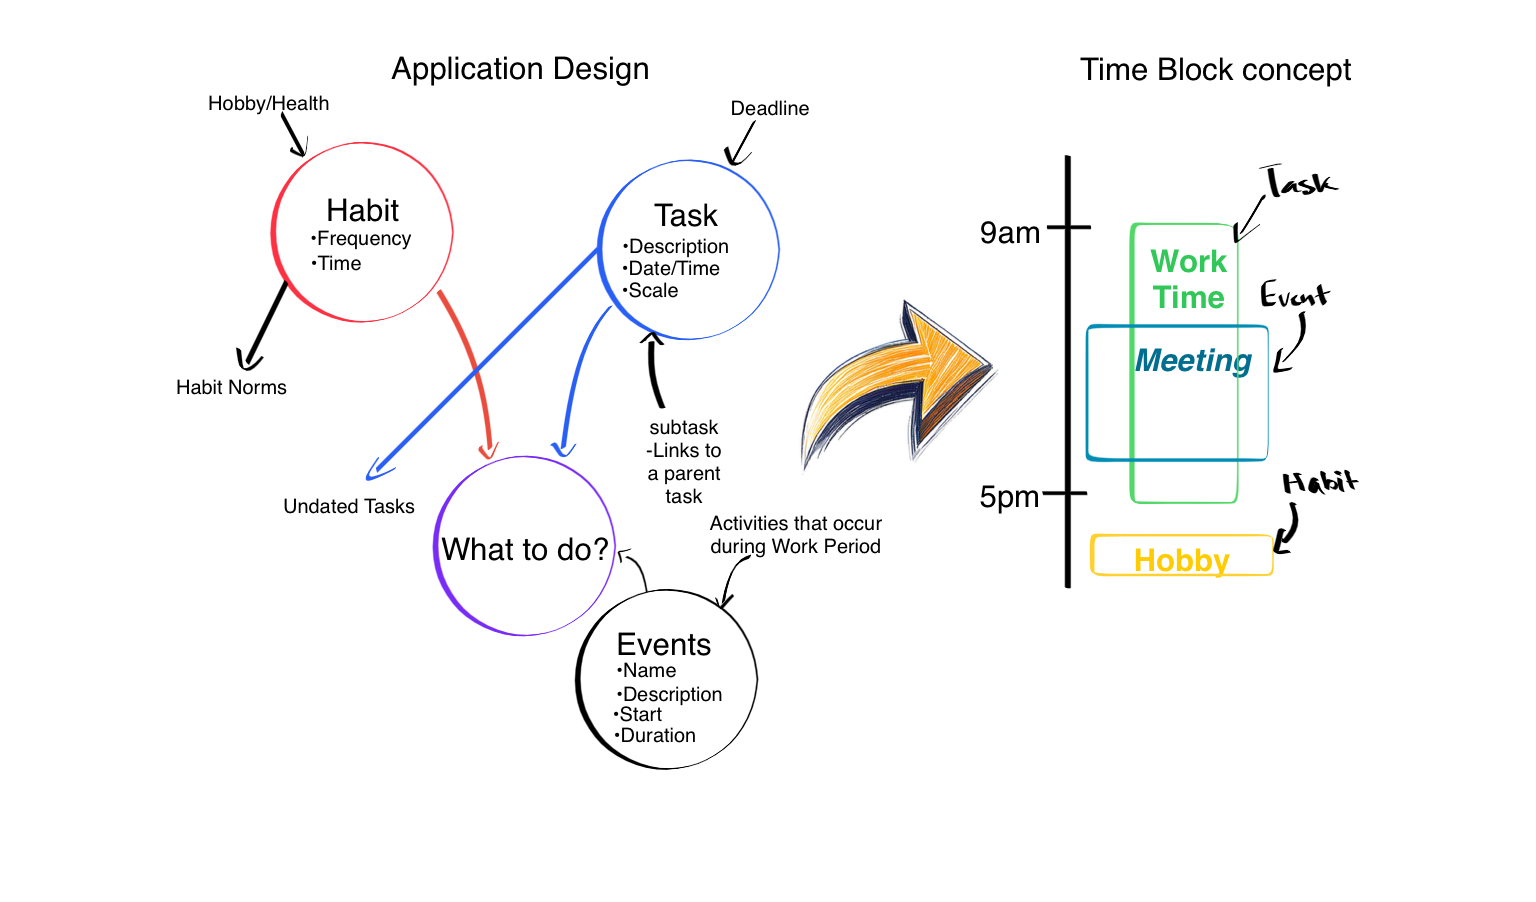
\includegraphics[width=\textwidth]{design_logic.png}
\end{frame}

\begin{frame}
  \frametitle{What's next?}
  % Confidence on on-time completion
  \begin{itemize}
    \item Prototype construction
  \end{itemize}
\end{frame}

\end{document}
